\documentclass{article}
\usepackage{pgfplots}
\pgfplotsset{compat=1.18}

\begin{document}

\begin{figure}[h]
    \centering
    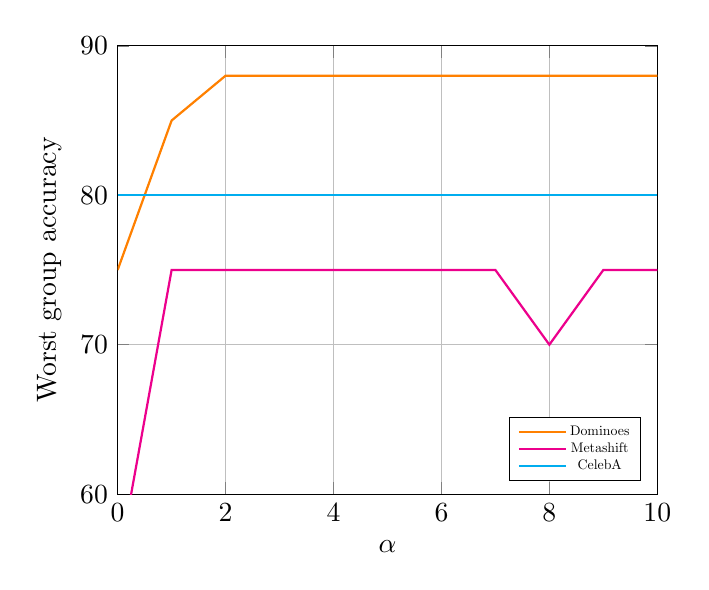
\begin{tikzpicture}
        \begin{axis}[
            xlabel=$\alpha$,
            ylabel=Worst group accuracy,
            legend pos=south east,
            grid=major,
            ymin=60,
            ymax=90,
            xmin=0,
            xmax=10,
            ytick={60,70,...,90},
            xtick={0,2,4,6,8,10},
            legend style={nodes={scale=0.5, transform shape}},
            ]
            \addplot[orange, thick] coordinates {
                (0,75) (1,85) (2,88) (3,88) (4,88) (5,88) (6,88) (7,88) (8,88) (9,88) (10,88)
            };
            \addlegendentry{Dominoes}
            
            \addplot[magenta, thick] coordinates {
                (0,55) (1,75) (2,75) (3,75) (4,75) (5,75) (6,75) (7,75) (8,70) (9,75) (10,75)
            };
            \addlegendentry{Metashift}
            
            \addplot[cyan, thick] coordinates {
                (0,80) (1,80) (2,80) (3,80) (4,80) (5,80) (6,80) (7,80) (8,80) (9,80) (10,80)
            };
            \addlegendentry{CelebA}
        \end{axis}
    \end{tikzpicture}
    \caption{Worst group accuracy on different datasets with respect to $\alpha$. $\alpha \geq 1$ is enough to increase worst group accuracy rapidly.}
\end{figure}

\end{document}